
%Developers and users can use a bounty to motivate developers to address an issue report. However, it still remains unclear how bounties affect the issue-addressing process.



In the previous sections, we studied the relationship between the issue-addressing likelihood, the bounty-usage frequency and the timing of proposing a bounty. However, there may exist more factors that potentially affect the issue-addressing likelihood. In this section, we conduct a deeper study on the relationship between other factors and the issue-addressing likelihood.
With a better understanding of this relationship, we can provide insights into how to use a bounty to improve the issue-addressing process.

\begin{figure*}[t]
\centering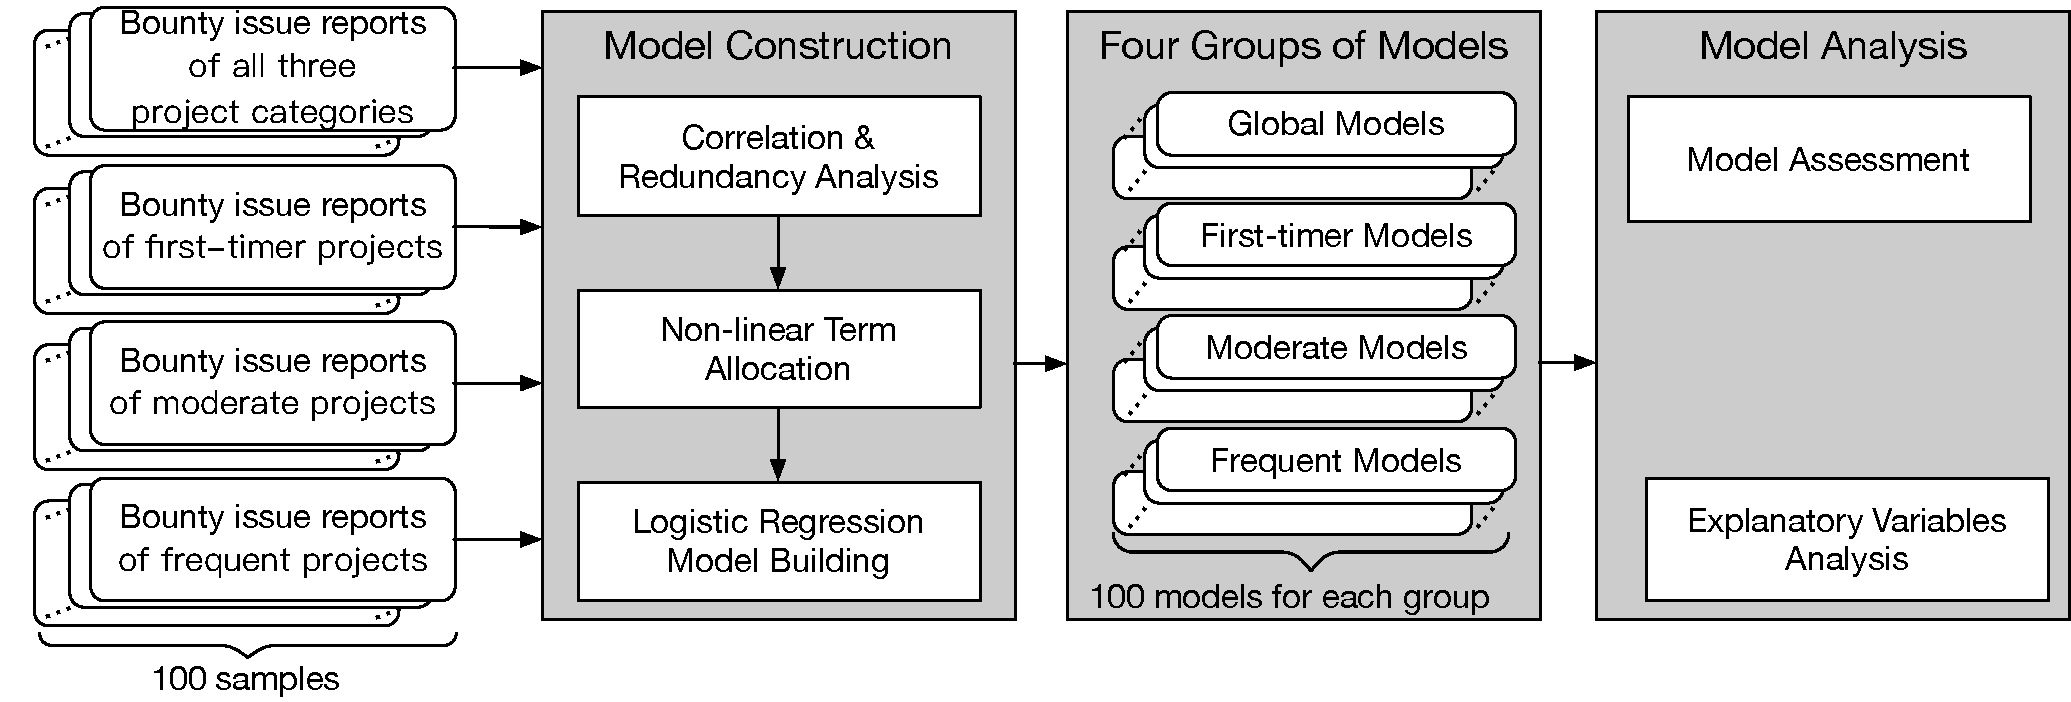
\includegraphics[width=17cm]{pics/rq3/rq3flow}
\vspace{-0.2in}
\caption{An overview of the model construction and analysis.}
\label{fig:rq3_flow}
\vspace{-0.1in}
\end{figure*}

\subsection{Approach}
In this section, we use the same data as in Section~\ref{rq1} to build logistic regression models to investigate the relationship between the studied factors and the issue-addressing likelihood.
Firstly, we build models on the entire set of bounty issue reports to understand the global relationship (referred to as the \textbf{global model}). Secondly, as we can see in Section~\ref{rq1}, the issue-addressing likelihood changes across project groups (i.e., the first-timer bounty-projects, the moderate bounty-projects, and the frequent bounty-projects). To understand the relationship within each project group, we build logistic regression models on the bounty issue reports of each group separately. To condense our writing, we refer to the model for the first-timer, moderate, and frequent bounty-projects as the \textbf{first-timer model}, \textbf{moderate model}, and \textbf{frequent model}, respectively.
We use the logistic regression modeling technique since it is a robust and highly interpretable technique, which has been applied successfully in software engineering before~\cite{wang2017understanding,mcintosh2016empirical}.
Figure~\ref{fig:rq3_flow} gives an overview of our approach.
Below, we elaborate on the studied factors, the processes of the model constructions, and the analysis of our models.

\subsubsection{Studied factors}
\begin{table*}[]
\centering
\footnotesize
\caption{The description of and rationale for the factors in the \emph{Issue report basic} and the \emph{Issue report bounty} dimensions. The factors which are marked with `*' are  time-dependent factors which are calculated at the time when the bounty is proposed}
\label{tab:factors1}

     \begin{tabular}{p{12em}p{29em}p{19em}}
     %\toprule
     \toprule
     \multicolumn{1}{l}{\textbf{Factor name}}  & \textbf{Description} & \multicolumn{1}{p{19em}}{\textbf{Rationale}} \\

     \midrule
     \multicolumn{3}{p{30em}}{\textbf{Issue report basic}}\\
     \midrule
      I\_content\_len*                  & The length of an issue report and its comments (in characters).  &\multirow{5}[-3]{19em}{\parbox{19em}{These factors reflect the amount of supportive information that an issue report has. Issue reports with more supportive information may help developers to address them.}} \\
%\cline{1-2}
     I\_code\_len* & The total length of the code snippets in an issue report and its comments (in characters). &  \\
%\cline{1-2}
      I\_code\_proportion*              & The proportion of code in an issue report and comments (i.e., $\frac{I\_code\_len}{I\_content\_len}$).\makecell{ \rule{0pt}{12pt} } &  \\
      \midrule
    I\_link\_cnt*                     & The number of links in an issue report and its comments. & \multirow{5}[-4]{19em}{\parbox{19em}{The discussion activities reflect the popularity of an issue report, which may have a relationship with the issue-addressing likelihood.}} \\
%\cline{1-2}
     I\_img\_cnt*                      & The number of images in an issue report and its comments. &  \\

%\cline{1-2}
     I\_cmnt\_cnt                     & The number of comments that an issue report received. & \\
%\cline{1-2}
	I\_participant\_cnt* & The number of participants in the discussion of an issue. & \\
%\cline{1-2}
     I\_cmnt\_per\_day\_mean* & The mean number of comments per day for an issue report. &  \\
 \midrule
     \textbf{Issue report bounty} & \multicolumn{2}{l}{\textbf{Description (d) - Rationale (r)}} \\
     \midrule
     I\_B\_days\_before\_bounty*  & \multicolumn{2}{p{48em}}{d: The number of days between the creation of an issue report and its first bounty.\newline r: Different timing of proposing bounties have relationship with the issue-addressing likelihood.} %\bigstrut
     \\
     %\hline
     %\midrule
      I\_B\_total\_value & \multicolumn{2}{p{48em}}{d: The total bounty value of the issue report. \newline r: A higher bounty may attract more developers.} \\
     %\midrule
     %\hline
      I\_B\_cnt    &  \multicolumn{2}{p{48em}}{d: The number of bounties that a bounty issue report has. \newline r: A higher number indicates that more backers are interested in getting this issue  addressed.} \\
      %\hline
     %\midrule
     I\_B\_has\_label  &  \multicolumn{2}{p{48em}}{d: Whether a bounty issue report is tagged with a bounty label. \newline r: A bounty label could help draw attention from the community, which may impact the issue-addressing likelihood. } \\
     %\hline
     %\midrule
      I\_B\_timing\_range*   & \multicolumn{2}{p{48em}}{d: The range of the timing of proposing the first bounty.                                                                                 \newline r: The timing of proposing a bounty has a relationship with the issue-addressing likelihood (see Section~\ref{rq2}).} \\
     \bottomrule
     %\hline
%\multicolumn{3}{l}{\textbf{Note:} The factors with `*' are collected at the time of proposing the first bounty for the issue report.}\bigstrut\\
     \end{tabular}%
     \vspace{-0.1in}
 \end{table*}%

\begin{table*}[ ]
\centering
%\tiny
\caption{The description of and rationale for the factors in the \emph{Project bounty} and the \emph{Backer experience} dimensions. The factors which are marked with `*' are  time-dependent factors which are calculated at the time when the bounty is proposed}
\label{tab:factors2}

     \begin{tabular}{p{10em}p{29em}p{21em}}
     \toprule
     \multicolumn{1}{l}{\textbf{Factor name}}  & \textbf{Description} & \multicolumn{1}{p{21em}}{\textbf{Rationale}} \\
     \midrule
     \multicolumn{3}{p{30em}}{\textbf{Project bounty}}\\
     \midrule
     P\_B\_I\_cnt*                     &  The total number of issue reports with at least one bounty of a project.  & \multicolumn{1}{r}{\multirow{5}[-5]{21em}{\parbox{21em}{These five factors reflect the bounty activity of the project. A different level of activity may have a different impact on the issue-addressing likelihood in the project.}}} \\
%\cline{1-2}
     P\_B\_paid\_cnt* & The total number of paid bounty issue reports of a project. &  \\
%\cline{1-2}
     P\_B\_open\_cnt*     &  The number of open bounty issue reports of a project.  &\\
%\cline{1-2}
     P\_B\_paid\_proportion* & The proportion of paid bounty issue reports of a project. &  \\
%\cline{1-2}
     P\_B\_total\_value* & The total value of the bounties of a project. &  \\
\midrule
      P\_B\_usage\_group                    &   The group of projects.                                                                                  & \multicolumn{1}{p{21em}}{Different groups of projects have different issue-addressing likelihoods (see Section~\ref{rq1}).} \\
     \midrule
     \multicolumn{3}{p{30em}}{\textbf{Backer experience}}\\
     \midrule
     Backer\_exp\_B\_median/sum/max\_value* & The median/sum/max value of bounties which the backers of this bounty have ever proposed in the past. & \multicolumn{1}{r}{\multirow{2}[1]{21em}{\parbox{21em}{Bounties from a backer who has proposed bounties often, or proposed high-value bounties in the past may attract more attention from developers.}}} t\\
%\cline{1-2}
     Backer\_exp\_B\_median/sum/max\_cnt* & The median/sum/max number of bounties which the backers of this bounty have ever proposed in the past. &  \\
     \midrule
     Backer\_role\_any\_insider* & Whether any of the backers who has ever contributed to the project.  & \multicolumn{1}{r}{\multirow{2}[1]{21em}{\parbox{21em}{A backer who has ever interacted with the project before may help the bounty attract more attention from the community.}}} \bigstrut\\
%\cline{1-2}
Backer\_role\_have\_reporter* & Whether the issue reporter is one of the backers for that issue report.\\
     \midrule

%\multicolumn{3}{l}{\textbf{Note:} The factors with `*' are collected at the time of proposing the first bounty for the issue report.}\\
     \end{tabular}%
\vspace{-0.2in}
 \end{table*}%

We consider 27 factors along 4 dimensions:
\begin{enumerate}
    \item \textbf{Issue report basic:} Eight factors which can estimate the length and the popularity of an issue report.
    \item \textbf{Issue report bounty:} Five factors which describe the bounty usage within a bounty issue report.
    \item \textbf{Project bounty:} Six factors which reflect the bounty usage within a project.
    \item  \textbf{Backer experience:}  Eight factors which capture the bounty experience of the backers of a bounty issue report.
\vspace{-0.01in}
\end{enumerate}

Table~\ref{tab:factors1} and Table~\ref{tab:factors2} summarize the description of and rationale behind the studied factors. The factors which are marked with `*' are time-dependent factors which are calculated at the time when the bounty is proposed.
Note that the factors in the project bounty, issue report basic, and backer experience dimensions cannot be changed by a backer who wants to propose a bounty. Hence we include these factors as control factors in our models.



\subsubsection{Model construction}
Similar to prior studies~\cite{gopi:2017,wang2017understanding,mcintosh2016empirical,kabinna2018examining}, we first removed correlated and redundant factors by using the Spearman rank correlation test and the redundancy analysis to avoid multicollinearity. We ended up with three factors in the project bounty dimension, six factors in the issue report basic dimension, four factors in the issue report bounty dimension, and three factors in the backer experience dimension.
Then we added non-linear terms in the model to capture the more complex relationship in the data by employing restricted cubic splines~\cite{Harrell:2006}.
Finally, we used the \code{rms} \code{R} package\footnote{\url{https://cran.r-project.org/web/packages/rms/index.html}} to implement our logistic regression models (i.e., the first-timer, moderate, frequent, and global models) based on 100 samples and ended up with 400 models. See our appendix~\cite{appendix} for more details about our model construction.

\subsubsection{Model analysis}
For each logistic regression model, we used the Area Under the Receiver Operating Characteristic Curve (i.e., \textit{AUC}) and a bootstrap-derived approach \cite{efron1986biased} to assess the explanatory power of the models following prior studies~\cite{mcintosh2016empirical,wang2017understanding,kabinna2018examining}. The AUC ranges from 0 to 1, with 0.5 being the performance of a random guessing model and a higher AUC meaning that the model has a higher ability to capture the relationships between the  explanatory factors and the response factor. To check whether the models are not overfitted, we calculate their \textit{optimism} values using a bootstrap-derived approach (with a small optimism value indicating that the model is not overfitted). 

To study the impact of each factor on the issue-addressing likelihood, we used the \textbf{anova} function in the R \textbf{rms} package to compute the Wald $\chi^2$ value.
The larger the Wald $\chi^2$ value of a factor is, the larger the impact of the factor on the issue-addressing likelihood.
We computed the Wald $\chi^2$ value for each factor for each model and used the median Wald $\chi^2$ value of each factor within a group to represent the impact of that factor in that group. %For the Wald $\chi^2$ value of factors in each group of models, please see the in Appendix\jy{ will add the specific section of appendix later}.

In addition, to further understand how a factor influences the value of the response variables, we used the \textbf{Predict} function in the \textbf{rms} R package to plot the estimated issue-addressing likelihood against a factor. Since all models across 100 samples showed similar patterns of influence for the factors, we randomly selected a sample as an example to build models and visualize the results (see Figure~\ref{fig:rq3_trend_global} and Figure~\ref{fig:rq3_trend_two}).
The analysis allows us to further understand how a factor affects the issue-addressing likelihood. %We hold the other factors at their median values when exploring a specific factor.
For the detailed results of our model analysis, such as the $\chi^2$ values, we refer the reader to our online appendix~\cite{appendix}.

%\begin{figure}[t]
%\centering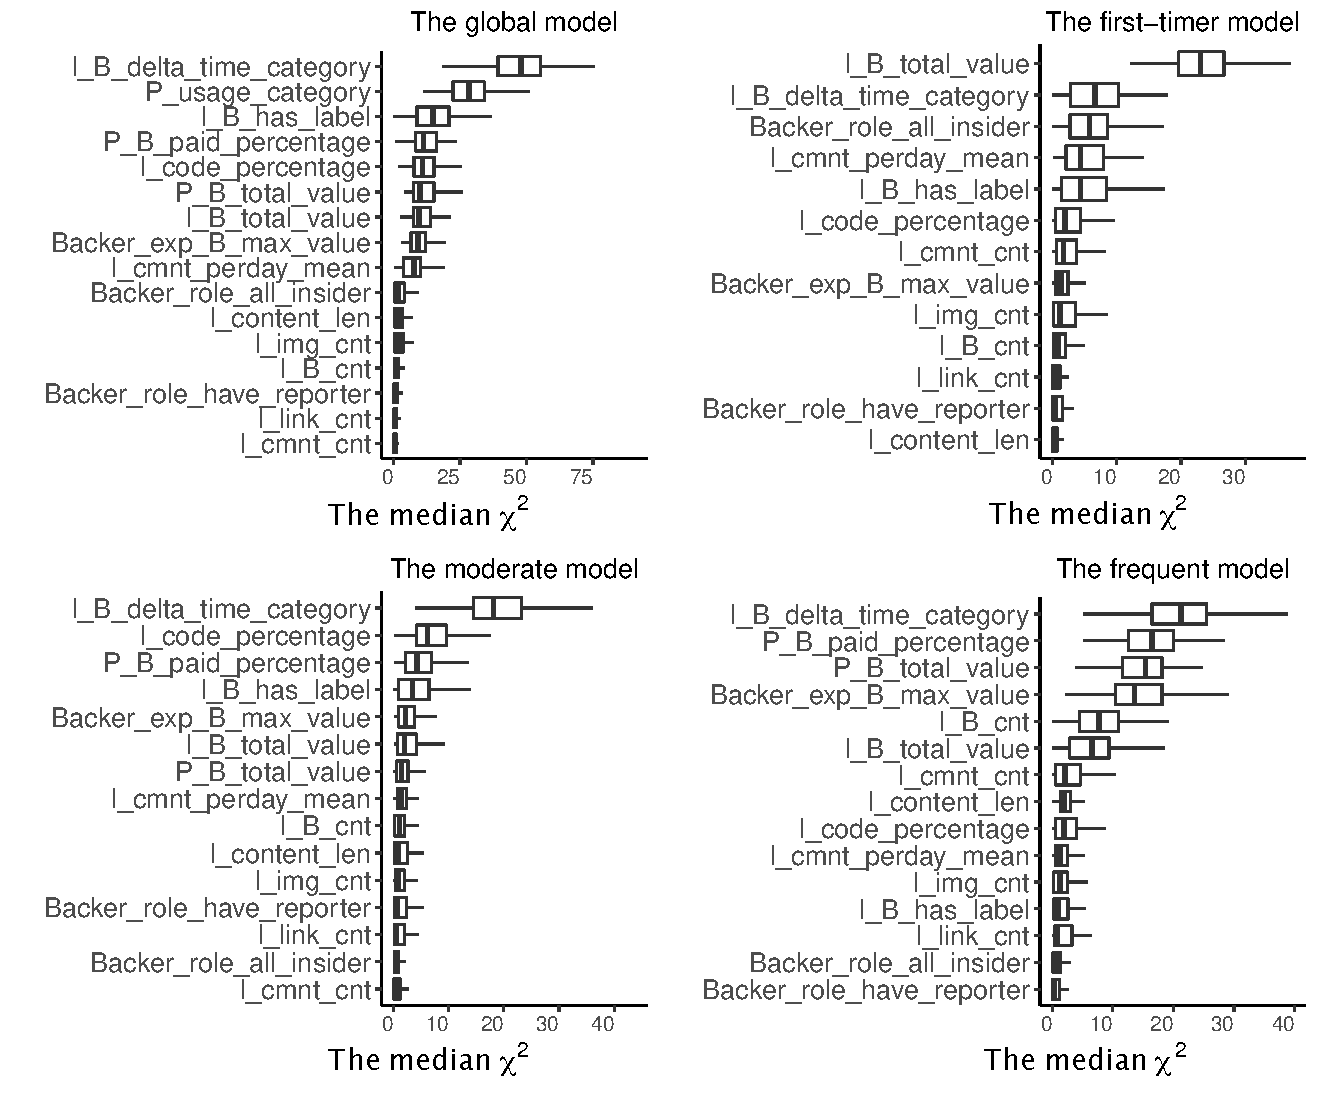
\includegraphics[width=\columnwidth]{pics/rq3/rq3_altogether}
%\caption{The distribution of the median Wald $\chi^2$ value of each factor in 100 samples for each group of models.}
%\label{fig:rq3_altogether}
%\end{figure}


\begin{figure}[t]
\centering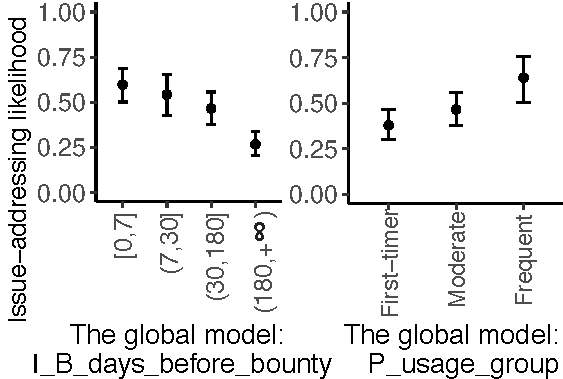
\includegraphics[width=0.7\columnwidth ]{pics/rq3/rq3_trend_global}
\caption{The plots show the relationship between the studied factors and the issue-addressing likelihood in the global models in the selected sample. For each plot, we adjusted all factors except the studied factor to their median value in the model and recomputed the issue-addressing likelihood. The grey area represents the 95\% confidence interval.}
\vspace{-0.1in}
\label{fig:rq3_trend_global}
\end{figure}

\begin{comment}
	
\begin{figure}[t]
\captionsetup[subfigure]{labelformat=empty}
    \centering
    \begin{subfigure}[t]{\columnwidth }
        \centering
        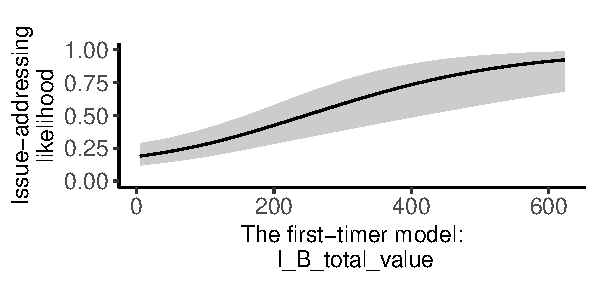
\includegraphics[width=\linewidth]{pics/rq3/split/rq3_trendCat1}
        \caption{}
		\label{fig:rq3_trendCat1}
    \end{subfigure}%

  \vspace{-0.2in}
    \begin{subfigure}[t]{\columnwidth}
        \centering
        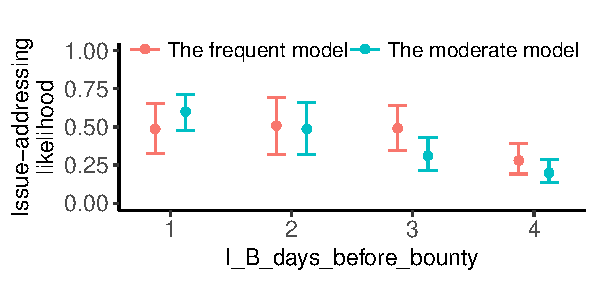
\includegraphics[width=\linewidth]{pics/rq3/split/rq3_trendMerge}
        \caption{}
          \label{fig:rq3_trendMerge}
    \end{subfigure}
  \vspace{-0.3in}
    \caption{The plots show the relationship between the studied factors and the issue-addressing likelihood in the first-timer, moderate and frequent models in the selected sample. For each plot, we adjusted all factors except the studied factor to their median value in the model and recomputed the issue-addressing likelihood. The grey area represents the 95\% confidence interval.
    }
    \label{fig:rq3_trend_two}
  \vspace{-0.1in}
\end{figure}

\end{comment}
\begin{figure}[t]
\centering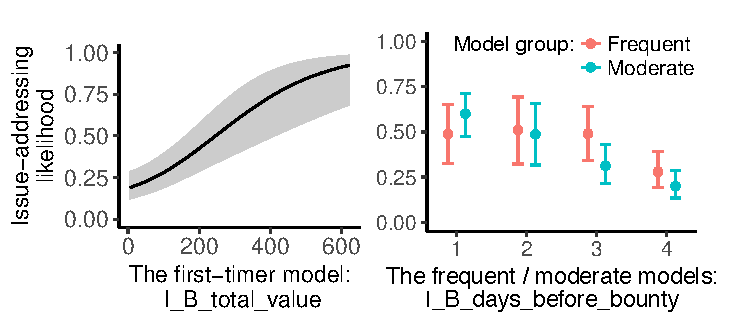
\includegraphics[width=1.03\columnwidth ]{pics/rq3/split/rq3_trendMergeMerge}
\caption{The plots show the relationship between the studied factors and the issue-addressing likelihood in the first-timer, moderate and frequent models in the selected sample. For each plot, we adjusted all factors except the studied factor to their median value in the model and recomputed the issue-addressing likelihood. The grey area represents the 95\% confidence interval.}
\vspace{-0.1in}
\label{fig:rq3_trend_two}
\end{figure}

 % Table generated by Excel2LaTeX from sheet 'Sheet1'
 \begin{table}[t]
   \centering
   \caption{The two most important factors, the median AUC and the median optimism (Opt.) values for our models.}
     \begin{tabular}{lp{8em}lcc}
     \toprule
     \textbf{Group} & \multicolumn{2}{c}{\rule{-14pt}{0pt} \textbf{Factor importance}} & \multicolumn{2}{c}{\rule{-11pt}{0pt}\textbf{Median}}\\
     \midrule
           & \multicolumn{1}{c}{\rule{-13pt}{0pt}$1^{st}$} & \multicolumn{1}{c}{\rule{-14pt}{0pt} $2^{nd}$} &  AUC & Opt.\\
     \midrule
     Global  &\rule{-13pt}{0pt} \textit{I\_B\_timing\_range} &\rule{-14pt}{0pt} \textit{P\_B\_usage\_group} &\rule{-11pt}{0pt} 0.72 & 0.02 \\
     
First-timer &\rule{-13pt}{0pt} \textit{I\_B\_total\_value} &\rule{-14pt}{0pt} \textit{I\_B\_timing\_range} &\rule{-11pt}{0pt} 0.74 & 0.03 \\

  Moderate &\rule{-13pt}{0pt} \textit{I\_B\_timing\_range} &\rule{-14pt}{0pt} \textit{I\_code\_proportion} &\rule{-11pt}{0pt} 0.71& 0.04 \\

   Frequent &\rule{-13pt}{0pt} \textit{I\_B\_timing\_range} &\rule{-14pt}{0pt} \textit{P\_B\_paid\_proportion} &\rule{-11pt}{0pt} 0.81 & 0.03 \\
     \bottomrule
     \end{tabular}%
   \label{tab:top3impFactors}%
   \vspace{-0.2in}
 \end{table}%


\subsection{Results}
\textbf{Our models explain our dataset well and have a reliable performance.} The median AUCs for each group of models are all at least 0.71 (see Table~\ref{tab:top3impFactors}), which indicates that our models explain the dataset well and the low median optimism values (between 0.02 and 0.04) indicate that our models do not overfit the dataset.

\textbf{In the global view, the timing of proposing the bounties and the bounty-usage frequency are the top two most important factors that impact the issue-addressing likelihood.} Table~\ref{tab:top3impFactors} shows the top two important factors (ranked by median Wald's $\chi^2$ value) in the global models across 100 samples.
\textit{I\_B\_timing\_range} (i.e., the range of the timing of proposing bounties) and \textit{P\_B\_usage\_group} (i.e., the group of projects' bounty-usage frequency) are the most important factors which contribute the most explanatory power to the models. This observation echoes our findings in Section~\ref{rq1} and~\ref{rq2} that the timing of proposing bounties and the bounty-usage frequency have a strong impact on the issue-addressing likelihood.

Figure~\ref{fig:rq3_trend_global} shows the relationship between the issue-addressing likelihood and the top two most important factors for the global model. \textit{I\_B\_timing\_range} has a negative relation with the issue-addressing likelihood, which indicates that issue reports for which bounties are proposed earlier have a higher likelihood of being addressed. This observation echoes with our findings in Section~\ref{rq2}.
%One possible explanation is that an early bounty may help the issue attract more attention from the community and increases the likelihood of an issue being addressed.
%GitHub's issue tracking system only lists the latest 25 issue reports at the first page by default and older issue reports could be buried by new issue reports. The earlier a bounty is proposed for an issue report, the higher the chance that the bounty will be recognized on the first several pages by the community.


\textbf{In the projects that use bounties moderately and frequently, issue reports are more likely to be addressed if backers propose bounties on an issue report earlier.} Table~\ref{tab:top3impFactors} shows that \textit{I\_B\_timing\_range} is the most important factor in the moderate and the frequent models. Especially in the moderate models, \textit{I\_B\_timing\_range} contributed more explanatory power than the other factors. For \textit{P\_B\_usage\_group}, we observe a positive relation with the issue-addressing likelihood in Figure~\ref{fig:rq3_trend_two}. One possible explanation is that projects with a higher bounty-usage frequency have more experience in using bounties which may increase the likelihood of a bounty being addressed. For example, the \code{eslint} project maintains a document on how bounties work\footnote{\url{%https://eslint.org/docs/developer-guide/contributing/working-on-issues
http://bit.ly/2Sql57n}}. The \code{eslint} project has 43 successful (i.e., closed-paid) and only one failed (i.e., open-unpaid) bounty issue report.


\textbf{The total bounty value of an issue report is the most important factor that impacts the issue-addressing likelihood in the first-timer bounty-projects, while it is less important in the projects in which bounties are used more frequently.} From Table~\ref{tab:top3impFactors}, we can see that \textit{I\_B\_total\_value} (i.e., the total bounty value of a bounty issue report) is the most important factor in the first-time model, while it is not as important in projects in which bounties are used more frequently. Figure~\ref{fig:rq3_trend_two} shows a positive relation between \textit{I\_B\_total\_value} and the issue-addressing likelihood of the first-time projects. This observation is compatible with our observations in Section~\ref{rq1} that successful bounty issue reports usually have much higher bounty values than failed bounty issue reports in the first-timer bounty-projects.




\rqbox{
In general, the timing of proposing bounties and the bounty-usage frequency are the top two most important factors that impact the issue-addressing likelihood. The total bounty value that an issue report has is the most important factor that impacts the issue-addressing likelihood in the first-timer bounty-projects, while it is not as important for projects in which bounties are frequently used.
}


